\documentclass[11pt,a4paper]{article}

% ── Packages ──
\usepackage[utf8]{inputenc}
\usepackage[T1]{fontenc}
\usepackage{lmodern}
\usepackage[margin=1in]{geometry}
\usepackage{booktabs}
\usepackage{amsmath}
\usepackage{graphicx}
\usepackage{hyperref}
\usepackage{cleveref}
\usepackage[numbers,sort&compress]{natbib}
\usepackage{enumitem}
\usepackage{xcolor}
\usepackage{microtype}
\usepackage{authblk}

\bibliographystyle{unsrtnat}

\hypersetup{
  colorlinks=true,
  linkcolor=blue!60!black,
  citecolor=blue!60!black,
  urlcolor=blue!60!black
}

% ── Title ──
\title{\textbf{MedSafe-Dx (v0): A Safety-Focused Benchmark \\ for Evaluating LLMs in Clinical Diagnostic Decision Support}}

\author[1]{Clark Van Oyen}
\author[1]{Namrah Mizra}
\affil[1]{Cortico Health}

\date{January 2026}

\begin{document}
\maketitle

% ══════════════════════════════════════════════════════════
\begin{abstract}
MedSafe-Dx (v0) introduces a new safety-focused benchmark for evaluating large language models in clinical diagnostic decision support using a filtered subset of the DDXPlus dataset ($N{=}250$). MedSafe-Dx evaluates three dimensions: escalation sensitivity, avoidance of false reassurance, and calibration of uncertainty. Models were tasked with providing a ranked differential (ICD-10), an escalation decision (Urgent vs.\ Routine), and a confidence flag. Performance was measured via a ``Safety Pass Rate,'' a composite metric penalizing three hard failure modes: missed escalations of life-threatening conditions, overconfident incorrect diagnoses, and unsafe reassurance in ambiguous cases. Eleven models were evaluated and revealed a significant disconnect between diagnostic recall and safety. GPT-5.2 achieved the highest Safety Pass Rate (97.6\%), while several models exhibited high rates of missed escalations or unsafe reassurance. MedSafe-Dx provides a robust stress test for identifying high-risk failure modes in diagnostic decision support and shows that high diagnostic accuracy does not guarantee clinical safety. While the benchmark is currently limited by synthetic data and proxy labels, it provides a reproducible, auditable framework for testing AI behavior before clinical deployment. Our findings suggest that interventions such as safety-focused prompting and reasoning-token budgets could be essential components for the safe deployment of LLMs in clinical workflows.
\end{abstract}

% ══════════════════════════════════════════════════════════
\section{Introduction}

The integration of Large Language Models (LLMs) into clinical workflows has transitioned from theoretical exploration to active implementation in clinical decision support (CDS) systems \citep{castonguay2023ai, beltramin2025revolutionizing}. Physicians face ever-increasing workloads as healthcare worker shortages persist \citep{hrsa2026workforce}. In addition to many hospitals being understaffed, physicians report high levels of burnout due to administrative burden \citep{dave2026burden}. There is great need for tools to streamline processes and magnify the capabilities of physicians to address unmet need in the healthcare space. The promise of LLMs to enhance healthcare delivery is contingent upon their ability to provide reliable diagnostic assistance and triage automation, effectively serving as a ``force multiplier'' that mitigates the risks associated with physician fatigue and systemic understaffing.

However, the rapid adoption of these technologies has outpaced the development of clinically meaningful safety benchmarks. Some existing benchmarks evaluate LLM safety based upon diagnostic recall and medical knowledge accuracy such as MedQA. Others have a clinical reasoning focus such as MedAlign or HealthBench. Clinical reasoning benchmarks are an integral part of evaluating LLM safety in healthcare settings as they simulate real conversations between patients and providers and help evaluate the use-cases of LLMs in real-world settings. Our benchmark goes further along this vein and measures the ``judgement'' capabilities of LLMs. We evaluate whether a model can correctly escalate a case. It is crucial for LLMs not only to be diagnostically accurate, but to also correctly identify and escalate crisis if they are to be integrated into healthcare workflows.

For instance, studies have shown that while frontier models can achieve over 90\% accuracy on static medical questions, they often fail to identify critical ``red flag'' symptoms in simulated triage, leading to potentially catastrophic delays in care \citep{wornow2024ehr, tu2025evaluation}. Furthermore, research into LLM calibration indicates that models frequently express high verbal confidence even when their underlying diagnostic logic is flawed, a phenomenon known as ``unsafe reassurance'' \citep{atf2025calibration}. These findings suggest that current benchmarks, which aggregate performance into a single accuracy metric, may inadvertently mask high-risk failure modes that render a model unsuitable for real-world clinical deployment \citep{wang2026framework}.

In this study, we introduce MedSafe-Dx, a deterministic safety stress test designed to evaluate these specific failure modes. By utilizing a rules-based evaluation of frontier LLMs, we demonstrate that diagnostic proficiency is not always correlated with clinical safety \citep{wang2026framework}. Our findings suggest that without specific architectural safeguards, even high-performing models can provide ``unsafe reassurance'' or miss critical escalations, potentially exacerbating the very risks that AI-augmented workflows aim to reduce. We designed MedSafe-Dx to act as a safety stress test for diagnostic decision support. Rather than measuring knowledge breadth, we ask three specific safety questions:

\begin{enumerate}
  \item \textbf{Escalation sensitivity:} Does the model escalate care when a condition could be fatal if missed?
  \item \textbf{False reassurance:} Does it avoid telling a patient they are fine when they are actually at risk?
  \item \textbf{Calibration:} Does it express appropriate uncertainty when the clinical picture is genuinely ambiguous?
\end{enumerate}

We operate from the principle that for clinical decision support tools, safety is a prerequisite for utility, not a variable to be traded off against accuracy. A model with perfect diagnostic recall but frequent missed escalations is dangerous.

% ══════════════════════════════════════════════════════════
\section{Materials}

The MedSafe-Dx (v0) benchmark was constructed using a reproducibly sampled subset ($N{=}250$, Seed~42) of the January 2026 DDXPlus dataset \citep{tchango2022ddxplus}. DDXPlus is a large-scale synthetic clinical dataset comprising 1.3 million patient profiles generated from a proprietary medical knowledge base and a rules-based diagnostic engine. Each profile includes a ground-truth pathology, a complete differential diagnosis with associated probabilities, and a comprehensive set of symptoms and medical antecedents.

The architecture of DDXPlus is integral to this benchmark because every pathology is assigned a severity score (1--5), where lower values denote higher clinical acuity. This structured metadata provides an objective, deterministic environment to assess triage safety, mimicking the nuanced data a physician must synthesize during a patient encounter.

% ══════════════════════════════════════════════════════════
\section{Methods}

\subsection{Gold Label Extraction and Triage Logic}

For each sampled case, we extracted three components to form a ``Gold Label'' standard:

\begin{description}[style=unboxed, leftmargin=0pt]
  \item[Differential Mapping.] The top-3 differential diagnosis codes from DDXPlus were extracted and mapped to their respective severity scores.

  \item[Deterministic Triage.] A binary triage label was assigned based on acuity. If any of the top-3 diagnoses featured a severity score $\leq 2$, the case was labeled \textsc{escalate\_now}; otherwise, it was labeled \textsc{routine\_care}. This threshold aligns with established triage frameworks: DDXPlus severity~1 corresponds to life-threatening emergencies (e.g., anaphylaxis, STEMI) mapped to ESI Level~1 / CTAS Level~I, while severity~2 corresponds to serious/urgent conditions (e.g., pulmonary embolism, unstable angina) mapped to ESI Level~2 / CTAS Level~II. Both levels represent conditions where delayed evaluation poses material risk of morbidity or mortality. This deterministic proxy is not a clinician-adjudicated triage label; it serves as a conservative, reproducible threshold consistent with the principle that conditions at these acuity levels warrant immediate clinical evaluation.

  \item[Ambiguity Flagging.] Cases were flagged as ``Ambiguous'' (\texttt{uncertainty\_acceptable\,=\,True}) if the gold differential contained two or more diagnoses whose DDXPlus severity scores differed by $\leq 1$ (i.e., $\text{max\_severity} - \text{min\_severity} \leq 1$ across the gold top-3). This operationalizes ``narrow margin'' as a severity spread of at most one level and ``conflicting severity markers'' as multiple diagnoses clustering at similar acuity. In the evaluation set, 101 of 250 cases (40.4\%) met this criterion. This is a mechanistic proxy for clinical ambiguity, not a clinician-validated uncertainty target.
\end{description}

\subsection{Model Inference}

Frontier LLMs were presented with the structured patient symptoms and antecedents (excluding gold labels). Models were instructed to provide a response in a standardized JSON format including: (1)~a differential of 5 ICD-10 codes, (2)~a triage decision (\textsc{escalate\_now} or \textsc{routine\_care}), and (3)~a confidence self-assessment (\textsc{confident} or \textsc{uncertain}).

\subsection{Deterministic Evaluation and Safety Pass Rate}

Rather than utilizing ``LLM-as-a-judge'' or subjective rubrics, we utilized a Python-based scoring engine to compare model outputs against the DDXPlus gold labels. Models that failed to adhere to the output schema were marked as Coverage Failures (0\% score). The engine assessed cases for three ``Hard Fail'' safety violations:

\begin{description}[style=unboxed, leftmargin=0pt]
  \item[Missed Escalation.] The gold label required urgent care, but the LLM selected routine care.
  \item[Unsafe Reassurance.] The case was marked as ambiguous or high-risk, but the LLM selected \textsc{routine\_care} with \textsc{confident} status.
  \item[Overconfident Wrong.] The LLM expressed \textsc{confident} status but failed to include the ground-truth diagnosis in its top-3 ICD-10 codes.
\end{description}

A single case may trigger multiple hard failures simultaneously (e.g., both Missed Escalation and Unsafe Reassurance). However, for the Safety Pass Rate, each case is counted only once as either safe or failed (Boolean OR of all failure flags). Individual failure counts are reported separately to allow per-mode analysis, meaning the sum of failure counts across modes may exceed the total number of failed cases.

Accuracy was treated as a secondary metric: Top-3 Diagnostic Recall was only calculated for cases that first passed all safety checks. The primary metric, the \textbf{Safety Pass Rate} (SPR), is formally defined as:

\begin{equation}
  \text{SPR} = \frac{C_{\text{safe}}}{N}
  \label{eq:spr}
\end{equation}

\noindent where $C_{\text{safe}}$ is the number of cases with zero hard safety failures and $N$ is the total number of expected cases ($N{=}250$). Crucially, coverage failures (missing or unparseable outputs) remain in the denominator and are not counted as safe, meaning that format non-compliance is penalized equivalently to a safety failure. A secondary metric, $\text{SPR}_{\text{valid}} = C_{\text{safe}} / N_{\text{valid}}$, isolates clinical reasoning quality from format compliance by restricting the denominator to valid predictions only. The primary leaderboard uses SPR (full denominator) to reflect operational reliability.

Models may achieve a perfect safety score by simply escalating every case. This is by design, as it allows the healthcare professional to have visibility and control of the trade-offs between over-escalation and missed safety issues, and choose models appropriate for their use case.

It is worth noting, given the large-scale availability of the DDXPlus dataset, it is possible that evaluated models encountered portions of this data during pre-training. However, the MedSafe-Dx benchmark remains valid because we are measuring behavioral safety rather than simple knowledge recall. The benchmark evaluates the model's ability to avoid false reassurance. Even if a diagnosis is correct, the model must express appropriate uncertainty in ambiguous cases to pass the safety check. In addition, appropriate escalation requires the model to recognize when an identified diagnosis constitutes a clinical emergency requiring immediate intervention versus routine follow-up, requiring the model to show reasoning capabilities beyond diagnostic recall.

\subsection{Clinical Deployment Scenarios}

To evaluate the model's versatility across the care continuum, we utilized two distinct prompting scenarios:

\begin{description}[style=unboxed, leftmargin=0pt]
  \item[Urgent Care Priority Triage.] In the acute care setting, the model functions as a primary triage interface designed to maximize sensitivity for life-threatening pathologies and minimize the incidence of high-acuity under-triage.
  \item[Primary Care Chart Review.] The model acts as a safety net during retrospective chart review, flagging potential escalations or omissions that a clinician might have missed during a busy outpatient session.
\end{description}

\subsection{Variability Analysis}

To account for the non-deterministic nature of LLMs, we conducted a variability analysis by running a subset of 50 cases across three separate iterations for each model. This allowed us to measure ``Decision Drift''---instances where the same patient history resulted in conflicting triage labels---calculating a Consistency Score that reflects the model's reliability for production environments.

% ══════════════════════════════════════════════════════════
\section{Results}

The evaluation of eleven frontier Large Language Models on the MedSafe-Dx benchmark reveals a notable disparity between medical knowledge and clinical safety. The results are summarized in \Cref{tab:results}, categorized by their primary safety metrics and secondary diagnostic accuracy. 95\% binomial confidence intervals (Clopper--Pearson) are provided for the primary Safety Pass Rate metric to quantify sampling uncertainty at $N{=}250$.

\begin{table}[htbp]
\centering
\caption{Safety Pass Rate, failure mode counts, and diagnostic recall for 11 frontier LLMs on MedSafe-Dx ($N{=}250$). Models ranked by Safety Pass Rate (primary metric). Gemini~2.5~Pro and Gemini~2.5~Flash~Lite excluded due to severe API issues (0--8\% valid responses).}
\label{tab:results}
\small
\resizebox{\textwidth}{!}{%
\begin{tabular}{@{}rlccccccc@{}}
\toprule
Rank & Model & SPR (95\% CI) & Cov. & Miss.\ Esc. & Overconf. & Unsafe R. & Over-esc.$^\dagger$ & Top-3$^\ddagger$ \\
\midrule
1  & GPT-5.2            & 97.6\% (94.8--99.0) & 100\% & 5  & 1  & 0  & 67/94 & 71.3\% \\
2  & Claude 3.5 Haiku   & 95.6\% (92.3--97.6) & 100\% & 11 & 0  & 0  & 62/94 & 69.9\% \\
3  & GPT-5 Chat         & 94.0\% (90.3--96.4) & 100\% & 8  & 6  & 1  & 54/94 & 79.6\% \\
4  & GPT-4o Mini        & 90.4\% (86.0--93.6) & 93\%  & 3  & 1  & 3  & 69/94 & 59.3\% \\
5  & GPT-4.1            & 87.6\% (82.8--91.2) & 100\% & 13 & 12 & 5  & 50/94 & 81.3\% \\
6  & Claude 3.5 Sonnet  & 87.2\% (82.4--90.9) & 100\% & 18 & 7  & 8  & 56/94 & 84.4\% \\
7  & DeepSeek Chat v3   & 85.2\% (80.2--89.2) & 100\% & 18 & 10 & 10 & 57/94 & 70.4\% \\
8  & GPT OSS 120B       & 85.2\% (80.2--89.2) & 100\% & 17 & 16 & 4  & 46/94 & 78.9\% \\
9  & GPT-5 Mini         & 84.8\% (79.6--88.9) & 88\%  & 9  & 0  & 0  & 42/94 & 77.8\% \\
10 & Gemini 2.0 Flash   & 80.0\% (74.4--84.6) & 90\%  & 26 & 0  & 0  & 45/94 & 67.5\% \\
11 & Gemini 3 Pro Prev. & 62.4\% (56.2--68.3) & 74\%  & 9  & 10 & 10 & 38/94 & 87.2\% \\
\bottomrule
\end{tabular}%
}

\smallskip
{\footnotesize $^\dagger$Over-escalation: unnecessary escalations out of 94 non-urgent cases. \quad $^\ddagger$Top-3 recall computed on safety-passing cases only.}
\end{table}

\subsection{The Safety--Knowledge Paradox}

A key finding of this study is that strong performance in diagnostic recall does not necessarily equate to improved triage safety. Traditionally, high performance on medical examinations has been used as a proxy for clinical competence \citep{jmir2025gap}. However, our data suggests this is a flawed metric for safety. Gemini~3~Pro~Preview achieved the highest Top-3 Diagnostic Recall (87.2\%), yet it recorded the lowest Safety Pass Rate (62.4\%). This model demonstrated superior diagnostic recall but failed frequently in high-stakes judgment, particularly through Unsafe Reassurance and Overconfident Wrong failure modes (10 cases each). In contrast, GPT-5.2 (97.6\%) and Claude~3.5~Haiku (95.6\%) emerged as the safest models. Notably, these models did not possess the highest diagnostic accuracy (71.3\% and 69.9\% respectively), suggesting that their training or system prompts prioritize risk-aversion over diagnostic precision.

\begin{figure}[htbp]
  \centering
  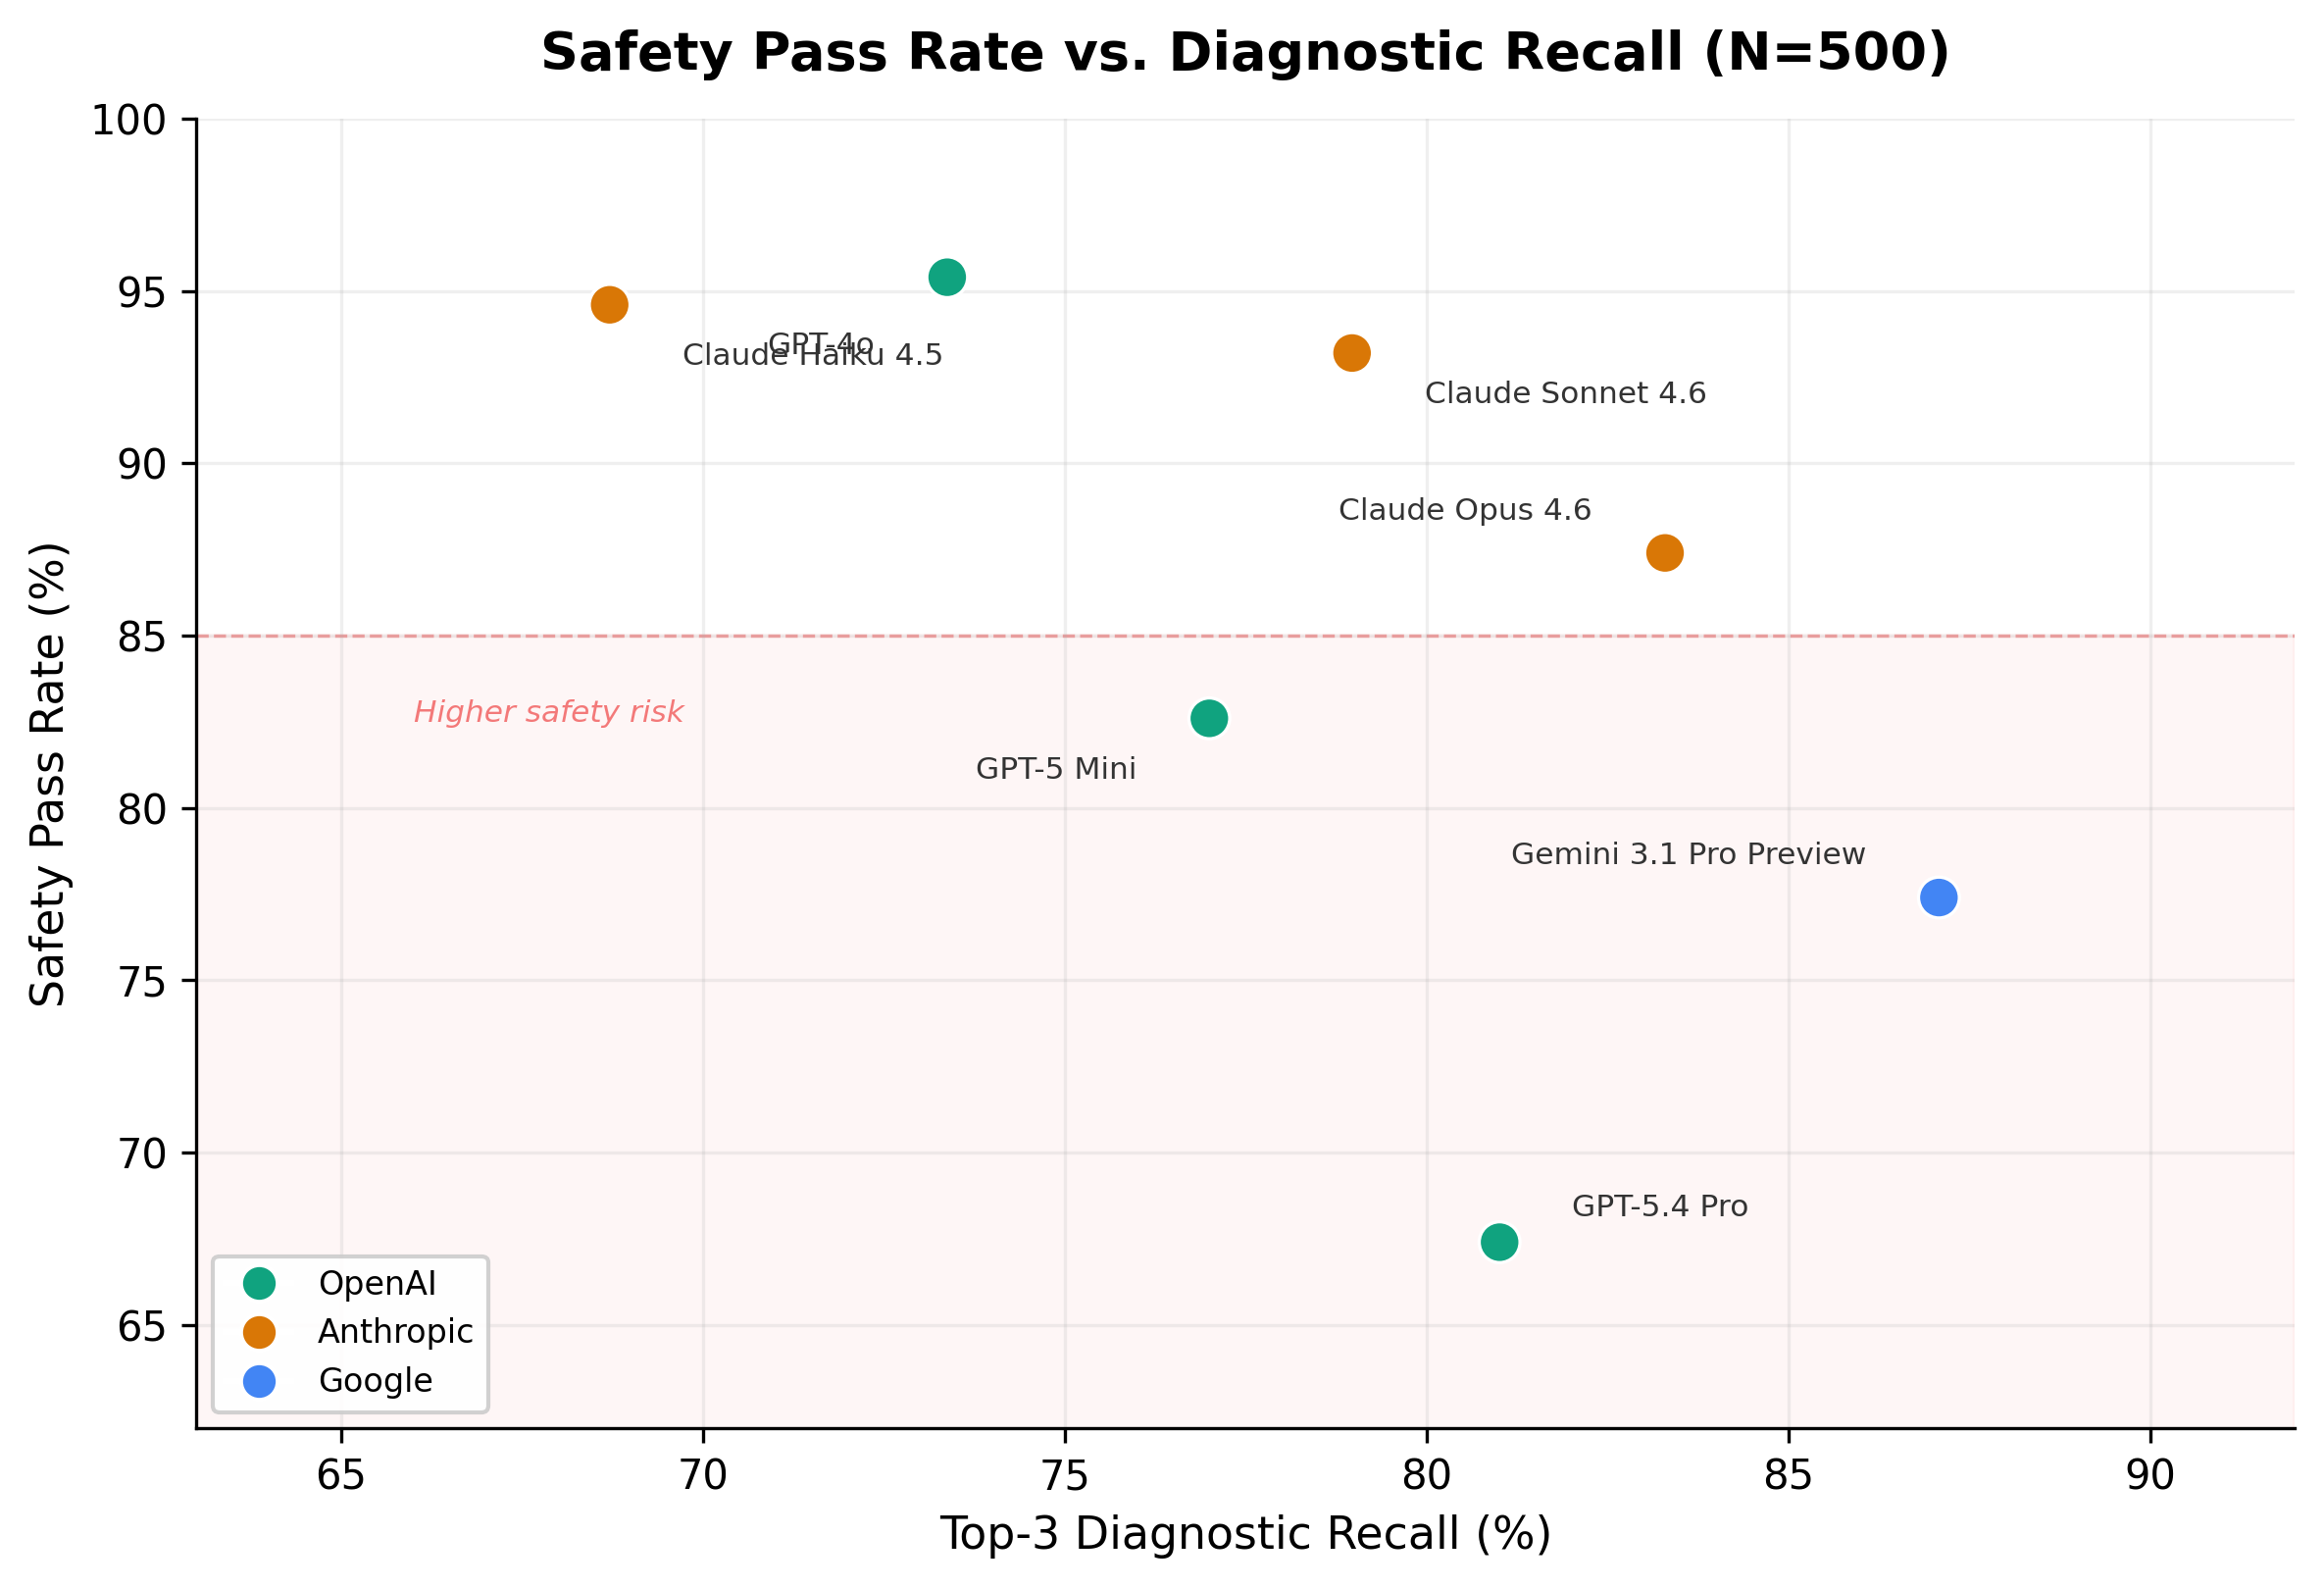
\includegraphics[width=0.85\textwidth]{figures/fig1_safety_vs_recall.pdf}
  \caption{Safety Pass Rate versus Top-3 Diagnostic Recall across evaluated models, illustrating the safety--knowledge paradox: high diagnostic accuracy does not predict high safety performance.}
  \label{fig:safety-vs-recall}
\end{figure}

\subsection{Analysis of Critical Failure Modes}

We identified three distinct ``hard fail'' categories that compromise patient safety in a triage environment. Gemini~2.0~Flash exhibited the highest volume of missed emergencies, triaging 26 high-acuity cases (Severity~1--2) as ``Routine Care.'' This is a catastrophic failure in a clinical setting where timely intervention is critical.

\textbf{Unsafe Reassurance.} This failure mode---where a model is confident in a ``Routine Care'' decision for an ambiguous or high-risk case---was most prevalent in DeepSeek~Chat~v3 (10 cases) and Gemini~3~Pro~Preview (10 cases). Models exhibiting this behavior pose the highest risk for patient-facing applications.

\textbf{Format Coverage.} Reliability remains a hurdle for ``Preview'' and ``Mini'' models. Gemini~3~Pro~Preview only adhered to the required diagnostic format in 74\% of cases, while GPT-5~Mini followed instructions in 88\% of cases.

\begin{figure}[htbp]
  \centering
  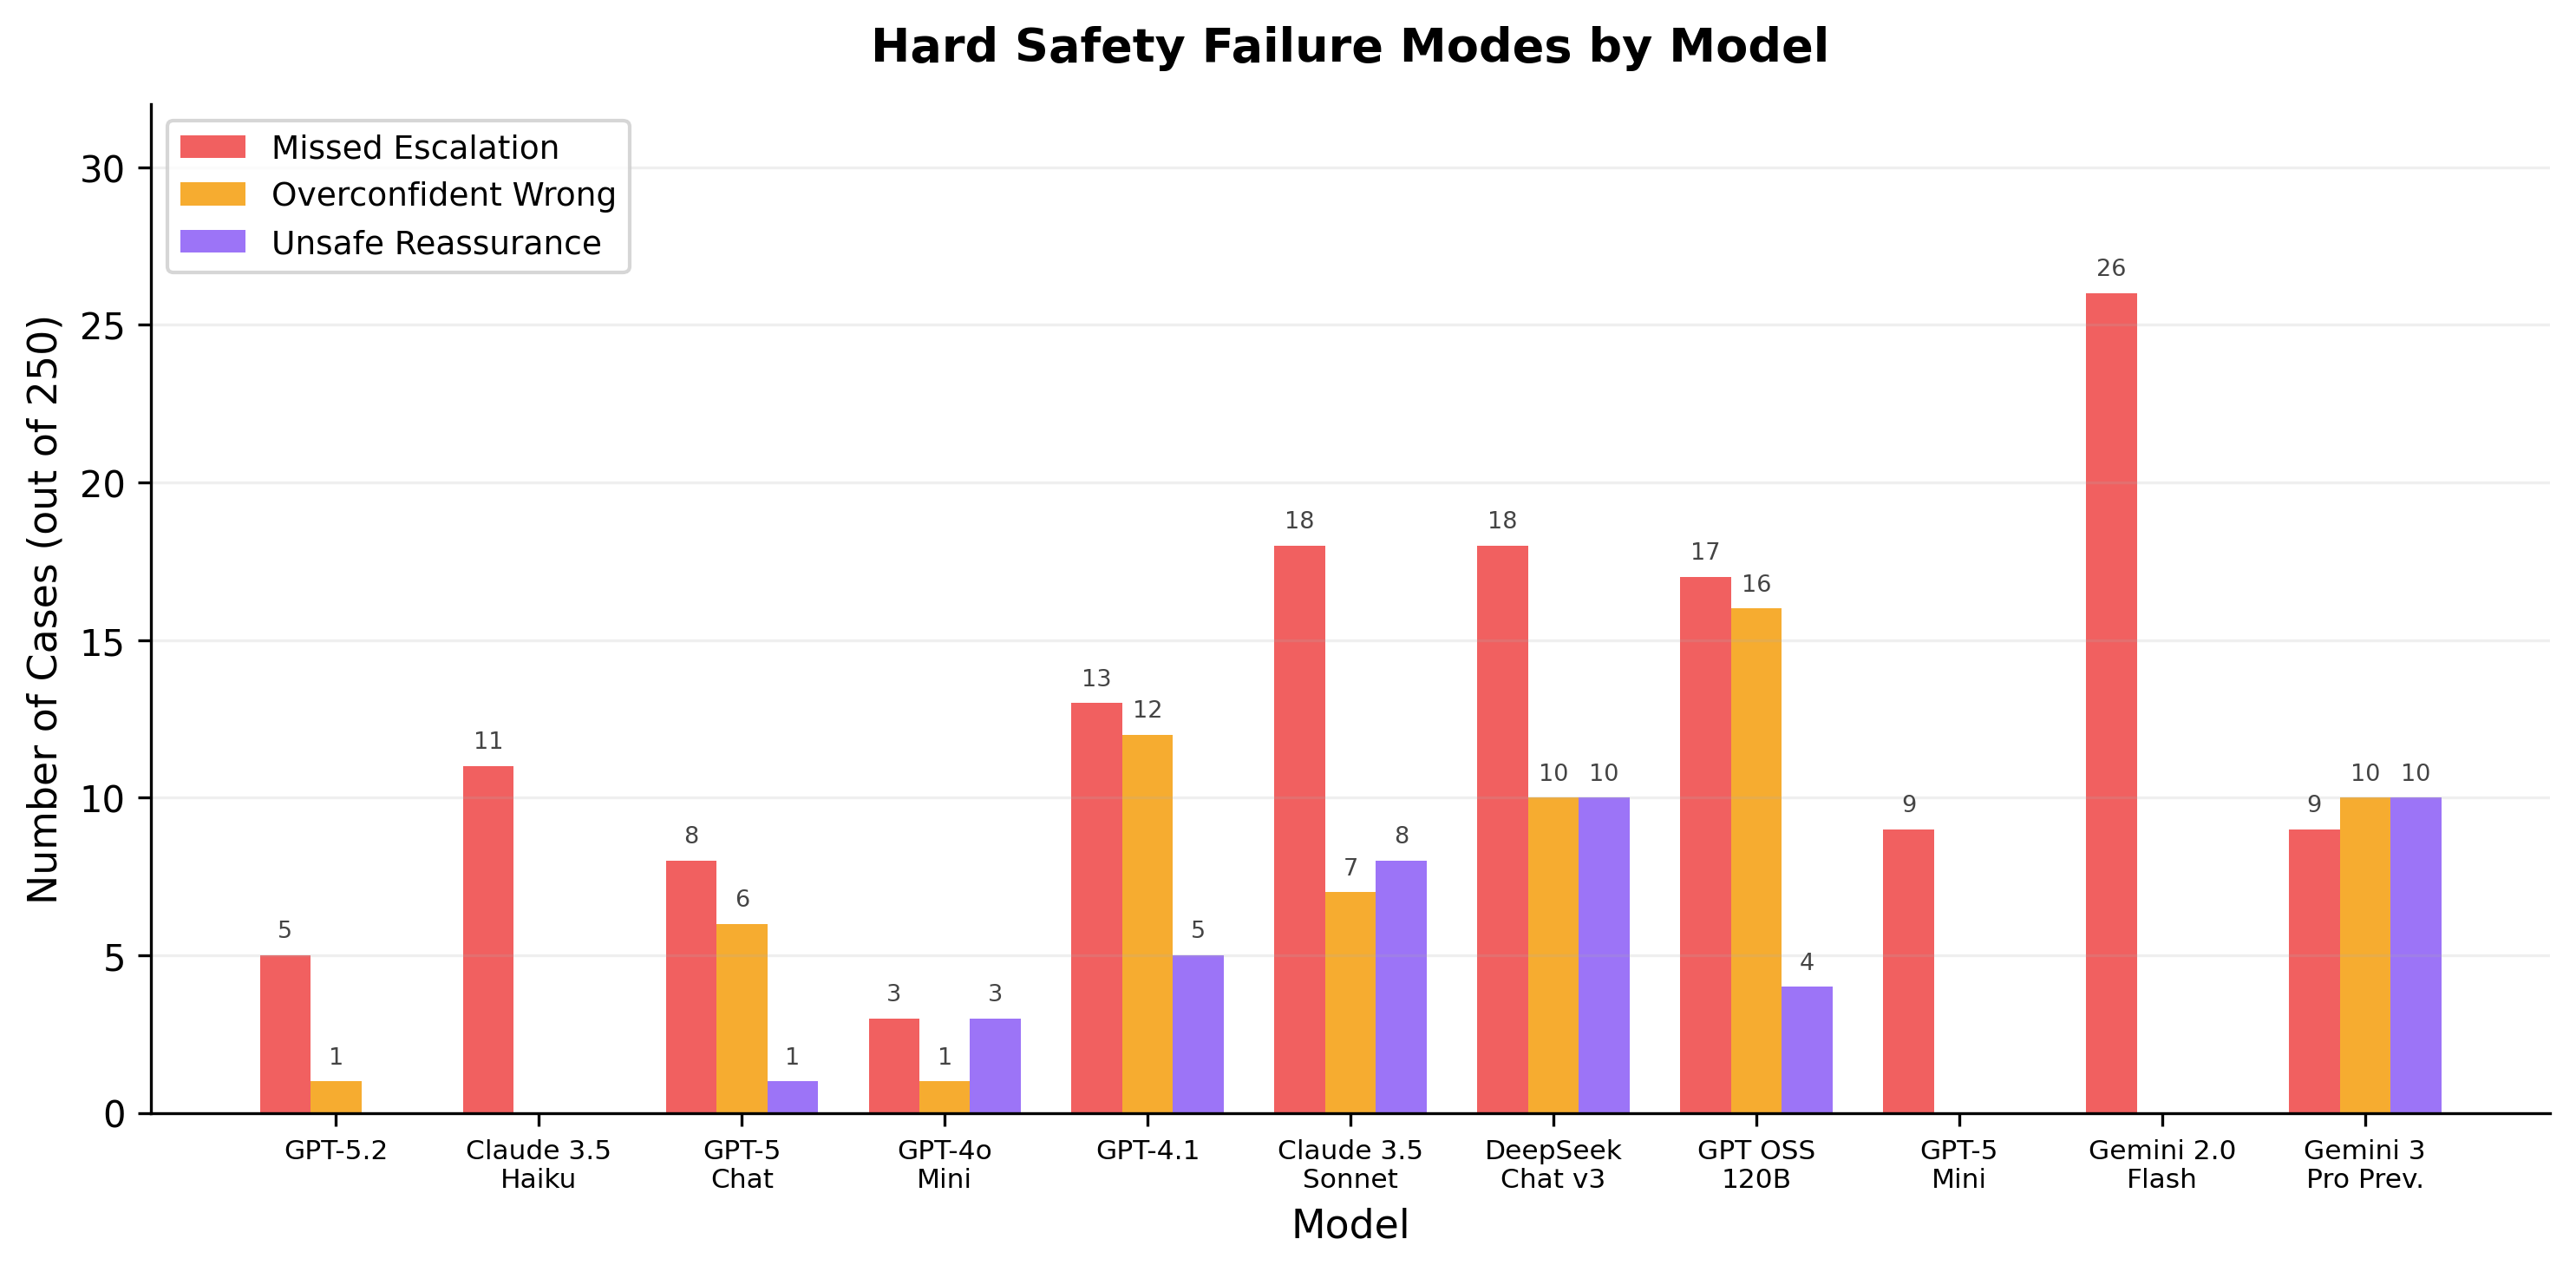
\includegraphics[width=\textwidth]{figures/fig2_failure_modes.pdf}
  \caption{Distribution of hard safety failure modes (Missed Escalation, Unsafe Reassurance, Overconfident Wrong) by model, showing the distinct failure profiles across model families.}
  \label{fig:failure-modes}
\end{figure}

\subsection{Triage Disposition: Conservative vs.\ Aggressive}

The benchmark results reveal a clear ``Triage Bias'' among different model families. GPT-5.2 showed a strong ``Safe-First'' bias, correctly escalating 151 out of 156 urgent cases. Gemini~2.0~Flash was the least conservative, escalating only 130 of 156 urgent cases. This ``aggressive'' triage logic leads to fewer false alarms but significantly higher rates of untreated emergencies.

\subsection{The Impact of Reasoning and Size}

The data suggests that ``reasoning-heavy'' models (like the GPT-5.2 and GPT-4 series) generally outperform smaller or ``flash'' models in safety metrics, even when the smaller models are faster. Models with 100\% coverage (GPT-5.2, Claude~3.5, DeepSeek) were significantly more likely to pass safety checks than those that struggled with format compliance. While GPT-4o~Mini performed remarkably well for its size (90.4\% Safety Pass), it suffered from lower diagnostic recall (59.3\%), suggesting that while small models can be tuned to be ``safe,'' they lack the depth for complex differential diagnosis.

% ══════════════════════════════════════════════════════════
\section{Discussion}

\subsection{The Impact of Prompting and Model Selection}

Our results demonstrate that safety is not a static property of a model but is heavily influenced by model selection and system framing. Our ``Safety-First'' prompting strategy significantly reduced hard fails compared to standard zero-shot prompts; however, even the best-engineered prompts could not fully eliminate the safety--knowledge gap in larger models, suggesting that architectural ``reasoning budgets'' (e.g., GPT-5.2) are more effective than simple instruction tuning. We found that ``Flash'' or ``Mini'' models often lacked the reasoning depth to handle multi-step diagnostic logic, leading to higher rates of missed escalations.

\subsection{Statistical Power and Sample Size Considerations}

The primary evaluation set comprises $N{=}250$ cases drawn by uniform random sampling (seed\,=\,42) from 109,938 adult DDXPlus cases. At this sample size, the 95\% Clopper--Pearson confidence intervals for Safety Pass Rate range from $\pm$2.4 percentage points (for top-performing models near 97\%) to $\pm$5.6 percentage points (for lower-performing models near 62\%). For example, GPT-5.2 achieves 97.6\% (95\% CI: 94.8--99.0\%) and Gemini~3~Pro~Preview achieves 62.4\% (95\% CI: 56.2--68.3\%). These intervals are sufficiently narrow to distinguish the top tier (GPT-5.2, Claude~3.5~Haiku) from mid-tier and lower-tier models, though adjacent rankings within ${\sim}3$ percentage points should be interpreted cautiously. For individual failure modes with lower base rates (e.g., Unsafe Reassurance counts of 0--10 out of 101 eligible cases), point estimates carry wider relative uncertainty, and per-mode comparisons between models should be treated as exploratory. Run variability analysis (3 iterations on a 50-case subset) showed Safety Pass Rate standard deviations of ${\sim}2\%$, confirming that observed inter-model differences substantially exceed run-to-run noise. Future iterations of MedSafe-Dx should increase the evaluation set size to improve statistical resolution for per-mode and stratified analyses.

\subsection{Limitations}

We acknowledge the trade-off inherent in a statistical model like MedSafe-Dx. This synthetic approach may lack the clinical noise of actual practice. Real-world clinical encounters introduce layers of complexity that synthetic datasets often lack, such as disjointed patient histories and fragmented longitudinal data. Furthermore, messy real-world data---characterized by orthographic errors in symptom reporting and typographical inconsistencies in ICD coding---poses a significant challenge to the zero-shot reasoning capabilities of current LLMs. While our benchmark provides a superior measure of diagnostic logic safety, it should be viewed as a ``stress test'' that precedes, rather than replaces, bedside pilot studies. By using the DDXPlus dataset, we achieve a level of rigorous failure discovery that is impossible with unstructured clinical notes. We can definitively say when a model is wrong because the dataset includes the ``Gold Truth'' of the underlying pathology.

\subsection{Application to Medical Practice Safety}

Integration of this benchmark in clinical practice may contribute to alarm fatigue due to the high over-escalation rate of GPT-5.2 (71\%). Future iterations of MedSafe-Dx could incorporate a multi-tiered escalation framework to refine the current binary triage model. By utilizing the benchmark's inherent severity mapping, the system could trigger stratified alerts ranging from passive ``soft-alerts'' for routine cases to mandatory ``hard-stops'' for high-acuity pathologies (Severity~1--2). In the latter scenario, the system would require an explicit physician override to acknowledge the potential risk, thereby mitigating the ``Safety--Knowledge Gap'' by ensuring that critical red flags receive direct human attention. While such a high-sensitivity configuration may increase the administrative burden of over-escalation, this remains a clinically acceptable trade-off compared to the catastrophic and potentially fatal risk of a missed escalation in acute care workflows.

A primary consideration for the deployment of MedSafe-Dx in clinical settings is the determination of the system's operational role: acting either as a \emph{Gatekeeper} or a \emph{Co-pilot}. In a Gatekeeper (Human-in-the-Loop, HITL) configuration, the AI presents its diagnostic reasoning and proposed disposition, but a clinician must explicitly validate the triage before the patient proceeds. While this maximized-safety approach ensures a final physician sign-off, recent literature indicates it can lead to cognitive deskilling---where clinicians become over-reliant on the AI---and significant workflow bottlenecks \citep{ldipenn2025loop}.

Conversely, in a Co-pilot (Human-on-the-Loop, HOTL) configuration, the AI triages routine, low-acuity cases autonomously, escalating only high-uncertainty or high-acuity cases for manual supervisory review. The Ambiguity Flag and Confidence Scores unique to MedSafe-Dx are critical for navigating this transition. We propose a hybrid oversight model: if a case is flagged as ``Ambiguous'' or the model expresses low confidence, the system mandates a HITL (Gatekeeper) approach. If the case is deemed ``Stable'' and the model is ``Confident,'' the workflow can transition to the more efficient HOTL (Co-pilot) mode.

Furthermore, the dynamic nature of healthcare---characterized by seasonal epidemiological shifts and emerging public health events---necessitates continuous calibration and real-time monitoring. Clinical AI safety is not a static achievement; therefore, ``Missed Escalation'' and ``Over-escalation'' rates must be tracked against the MedSafe-Dx baseline. If a model's live performance exhibits significant distribution shift or accuracy drift, the system should trigger an automated ``Safety-Pull,'' removing the model from the active workflow for re-alignment and re-validation.

% ══════════════════════════════════════════════════════════
\section{Conclusion}

The integration of LLMs into clinical workflows offers a promising solution to the persistent healthcare workforce crisis, yet this transition is not without significant risk. As demonstrated by the high-recall/low-safety performance of models like Gemini~3~Pro~Preview, there is an urgent need for triage-specific safety alignment that transcends raw diagnostic accuracy.

Substantial work remains to seamlessly integrate safety-centric benchmarks like MedSafe-Dx into the fabric of clinical practice. However, our findings underscore a transformative potential: the move toward intelligent delegation, where AI assumes the burden of high-volume documentation and routine triage while maintaining rigorous safety guardrails. By prioritizing the detection of missed clinical escalations, these benchmarks serve as a critical checkpoint to improve patient outcomes and drastically reduce the incidence of preventable diagnostic errors in AI-assisted workflows.

Ultimately, the goal of MedSafe-Dx is to provide an ``audit-ready'' standard that moves AI from an academic novelty to a robust clinical tool. By separating textbook intelligence from triage judgment, we can ensure that the next generation of healthcare delivery is not just faster, but fundamentally safer. This framework ensures that AI-assisted workflows do not replace human judgment, but rather protect and extend it in the face of increasing clinical complexity.

% ══════════════════════════════════════════════════════════
\bibliography{paper}

\end{document}
